% =====================================================================
%  Chapter 4 — The \idxw{Population} We Are Accountable For
% =====================================================================

\chapter{The Population We Are Accountable For}
\label{ch:population}

A programme that cannot say what it is trying to cover cannot be managed,
because it has no denominator. This chapter fixes the denominator, and in
doing so it produces the single most important number in the book: for the
class of objects that can destroy a city, the near-Earth object catalogue is
essentially complete, and the gap is not discovery. It is accounting.

\section{The three populations}

The catalogue is usually quoted as one number, 43,212 known near-Earth objects
as of 22 November 2026. That number is a poor management unit, because it
mixes objects that can level a city with objects that are less likely to
damage a building. Three populations matter, and they are worth separating.

\begin{table}[!htbp]
\centering
\small
\caption{The catalogue by the population that matters, with the annual arrival
rate. Source: NASA CNEOS discovery statistics, data current 22 November 2026.}
\label{tab:populations}
\begin{tabularx}{\textwidth}{@{}P{1.11in}P{0.73in}P{0.87in}Y@{}}
\toprule
\rowcolor{panel}
\textbf{Population} & \textbf{Known} & \textbf{Arriving} & \textbf{What it means} \\
\midrule
All near-Earth objects & 43,212 & 3,383 a year & dominated by objects too
small to matter \\
\rowcolor{panel}
140 m and larger & 11,725 & 342 a year & the population\idx{Population} a defender is
accountable for \\
1 km and larger & 883 & 2 a year & essentially complete \\
\bottomrule
\end{tabularx}
\end{table}

The 140-metre class is the working population\idx{Population}, and the choice of 140~metres is
not arbitrary. It is the size at which an object delivers enough energy to
destroy a city on its own, and it is also the threshold the discovery
statistics themselves use. The class contains 11,725 objects, which is 27.1 per
cent of the whole catalogue. Its arrival rate is falling: 441 in 2022, 431 in
2023, 397 in 2024 and 342 in 2025, because the large objects are running out
and the easy ones have already been found. At that rate the remaining
undeclared population\idx{Population} of this class is small and finite.

\begin{figure}[!htbp]
\centering
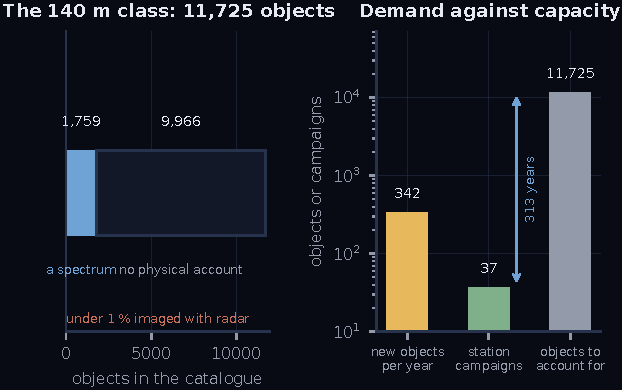
\includegraphics[width=\textwidth]{../figures/fig_accountability.pdf}
\caption{The population that is catalogued but not accounted for, and the
demand against which a single characterisation station's capacity has to be
read. The right-hand panel is logarithmic: the backlog is three hundred times
the station's annual service rate.}
\label{fig:accountability}
\end{figure}

\section{How many of them have an account}

The characterisation\idx{Characterisation} record for this population is thin. The survey of the
field's characterisation\idx{Characterisation} capability records that only about fifteen per cent
of near-Earth objects have had a spectrum measured, and that fewer than one
per cent have been imaged with radar. Applied to the 140-metre class, those
two figures give about 1,759 objects with a spectrum and fewer than about 120
with a radar image. The remainder, about 9,966 objects, have no physical
account at all.

\begin{table}[!htbp]
\centering
\small
\caption{The physical accounts that exist for the 140-metre class, as far as
the published figures reach.}
\label{tab:accounts}
\begin{tabularx}{\textwidth}{@{}P{1.60in}P{0.96in}Y@{}}
\toprule
\rowcolor{panel}
\textbf{Account} & \textbf{Objects} & \textbf{What it settles} \\
\midrule
A spectrum & about 1,759 & composition, taxonomy, and an albedo prior \\
\rowcolor{panel}
A radar image & fewer than about 120 & shape, spin state, and in principle
mass \\
A resolved shape model & a few dozen & the volume that the energy chain
starts from \\
\rowcolor{panel}
A mass & very few & the density, and with it the last term in
\eqref{eq:dlne} \\
\bottomrule
\end{tabularx}
\end{table}

The last row is the one that should worry a programme manager most. A
resolved shape model gives the volume; the mass gives the density; the
density is the other factor of three in \eqref{eq:dlne}. A catalogue in which
one object in seven has a spectrum and one in a hundred has a radar image is
not a catalogue of known threats. It is a catalogue of known objects.

\section{The managerial consequence}

The arithmetic in the previous three sections produces a conclusion that
determines the shape of the whole proposal, and it is a conclusion about
\emph{what kind of thing} the capability should be.

If the gap were a discovery gap, the right response would be more survey
capacity: a larger aperture, a longer telescope, a faster cadence. The
published survey record shows that the discovery side is not the bottleneck
for the class that matters. The 140-metre population is nearly complete in
discovery and nearly untouched in characterisation. Building more survey
capacity adds objects to a queue that already cannot be served.

If the gap were a capacity gap --- if there were simply too many objects to
characterise for any instrument to keep up --- then the response would be to
build a census machine and accept the cost. It would not be a census machine,
because the arithmetic rules it out. A fixed station needs a 90-degree sweep
of its baseline orientation to deliver the two orthogonal measurements an
interferometric position requires, and the Moon's rotation takes 6.83 days
to deliver that sweep. Allowing thirty per cent of the time for overhead, one
station runs about 37 campaigns a year. Against an arrival rate of 342
objects a year for the hazard class, that is 10.9 per cent of the flow, and
against the 11,725 known objects it is a clearance time of 313 years.

\begin{keytakeaways}
\item The working population is the 11,725 known objects larger than about
140 metres, and its discovery is essentially complete.
\item About 1,759 have a spectrum, fewer than about 120 have a radar image,
and about 9,966 have no physical account at all.
\item More survey capacity would add objects to a queue that cannot be served;
the bottleneck is characterisation\idx{Characterisation}, not detection.
\item One station runs about 37 campaigns a year, which is 10.9 per cent of
the annual flow and a 313-year clearance of the known catalogue, so the
capability must be a triage and not a census.
\end{keytakeaways}

The conclusion follows directly, and it is the load-bearing structural claim of
the book: \textbf{for the hazard class, the gap is accounting, not
discovery}. A capability for this population therefore cannot be justified by
how much it finds, and it cannot be justified by the size of the backlog.
It has to be justified by the decisions it changes --- which is to say, by the
objects whose characterisation actually alters an outcome. That is a
narrower claim than ``characterise the catalogue'', and Chapter 30 turns it
into a rule.

\begin{figure}[!htbp]
\centering
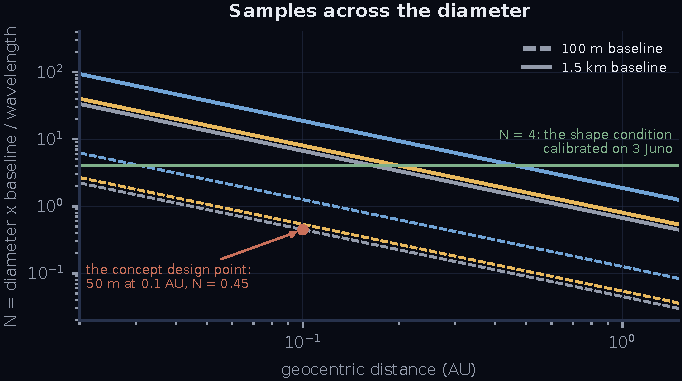
\includegraphics[width=\textwidth]{../figures/fig_samples.pdf}
\caption{Samples across the diameter against baseline and distance. A single
100-metre baseline never reaches four samples for the 50-metre class at
0.2 astronomical units, and the proposed array is what closes the gap.}
\label{fig:samples}
\end{figure}
